\section{Introduction}
Building distributed frameworks to facilitate Machine Learning on large and growing datasets has is a key data management challenge with significant interest in both industry and academia~\cite{bdas, alexandrov2014stratosphere, crotty2014tupleware, tensor}.
Despite a number of breakthroughs in reducing training time, predictive modeling can still be a tedious and time-consuming task for an analyst. 
Data often arrive \emph{dirty}, including missing, incorrect, or inconsistent attributes, and analysts widely report that data cleaning and other forms of pre-processing account for up to 80\% of their effort~\cite{nytimes, kandel2012}.
While data cleaning is an extensively studied problem, the predictive modeling setting poses a number of new challenges: (1) high dimensionality can amplify even a small amount of erroneous records~\cite{xiaofeature}, (2) the complexity can make it difficult to trace the consequnces of an error, and (3) there are often subtle technical correctness conditions (e.g., independent and identically distributed) that can be violated by data cleaning.
Consequently, techniques that have been designed for traditional SQL analytics may be inefficient or even unreliable.
In this paper, we study the relationship between data cleaning and model training workflows and explore how to apply existing data cleaning approaches with provable guarantees.

\begin{figure}[t]
\centering
 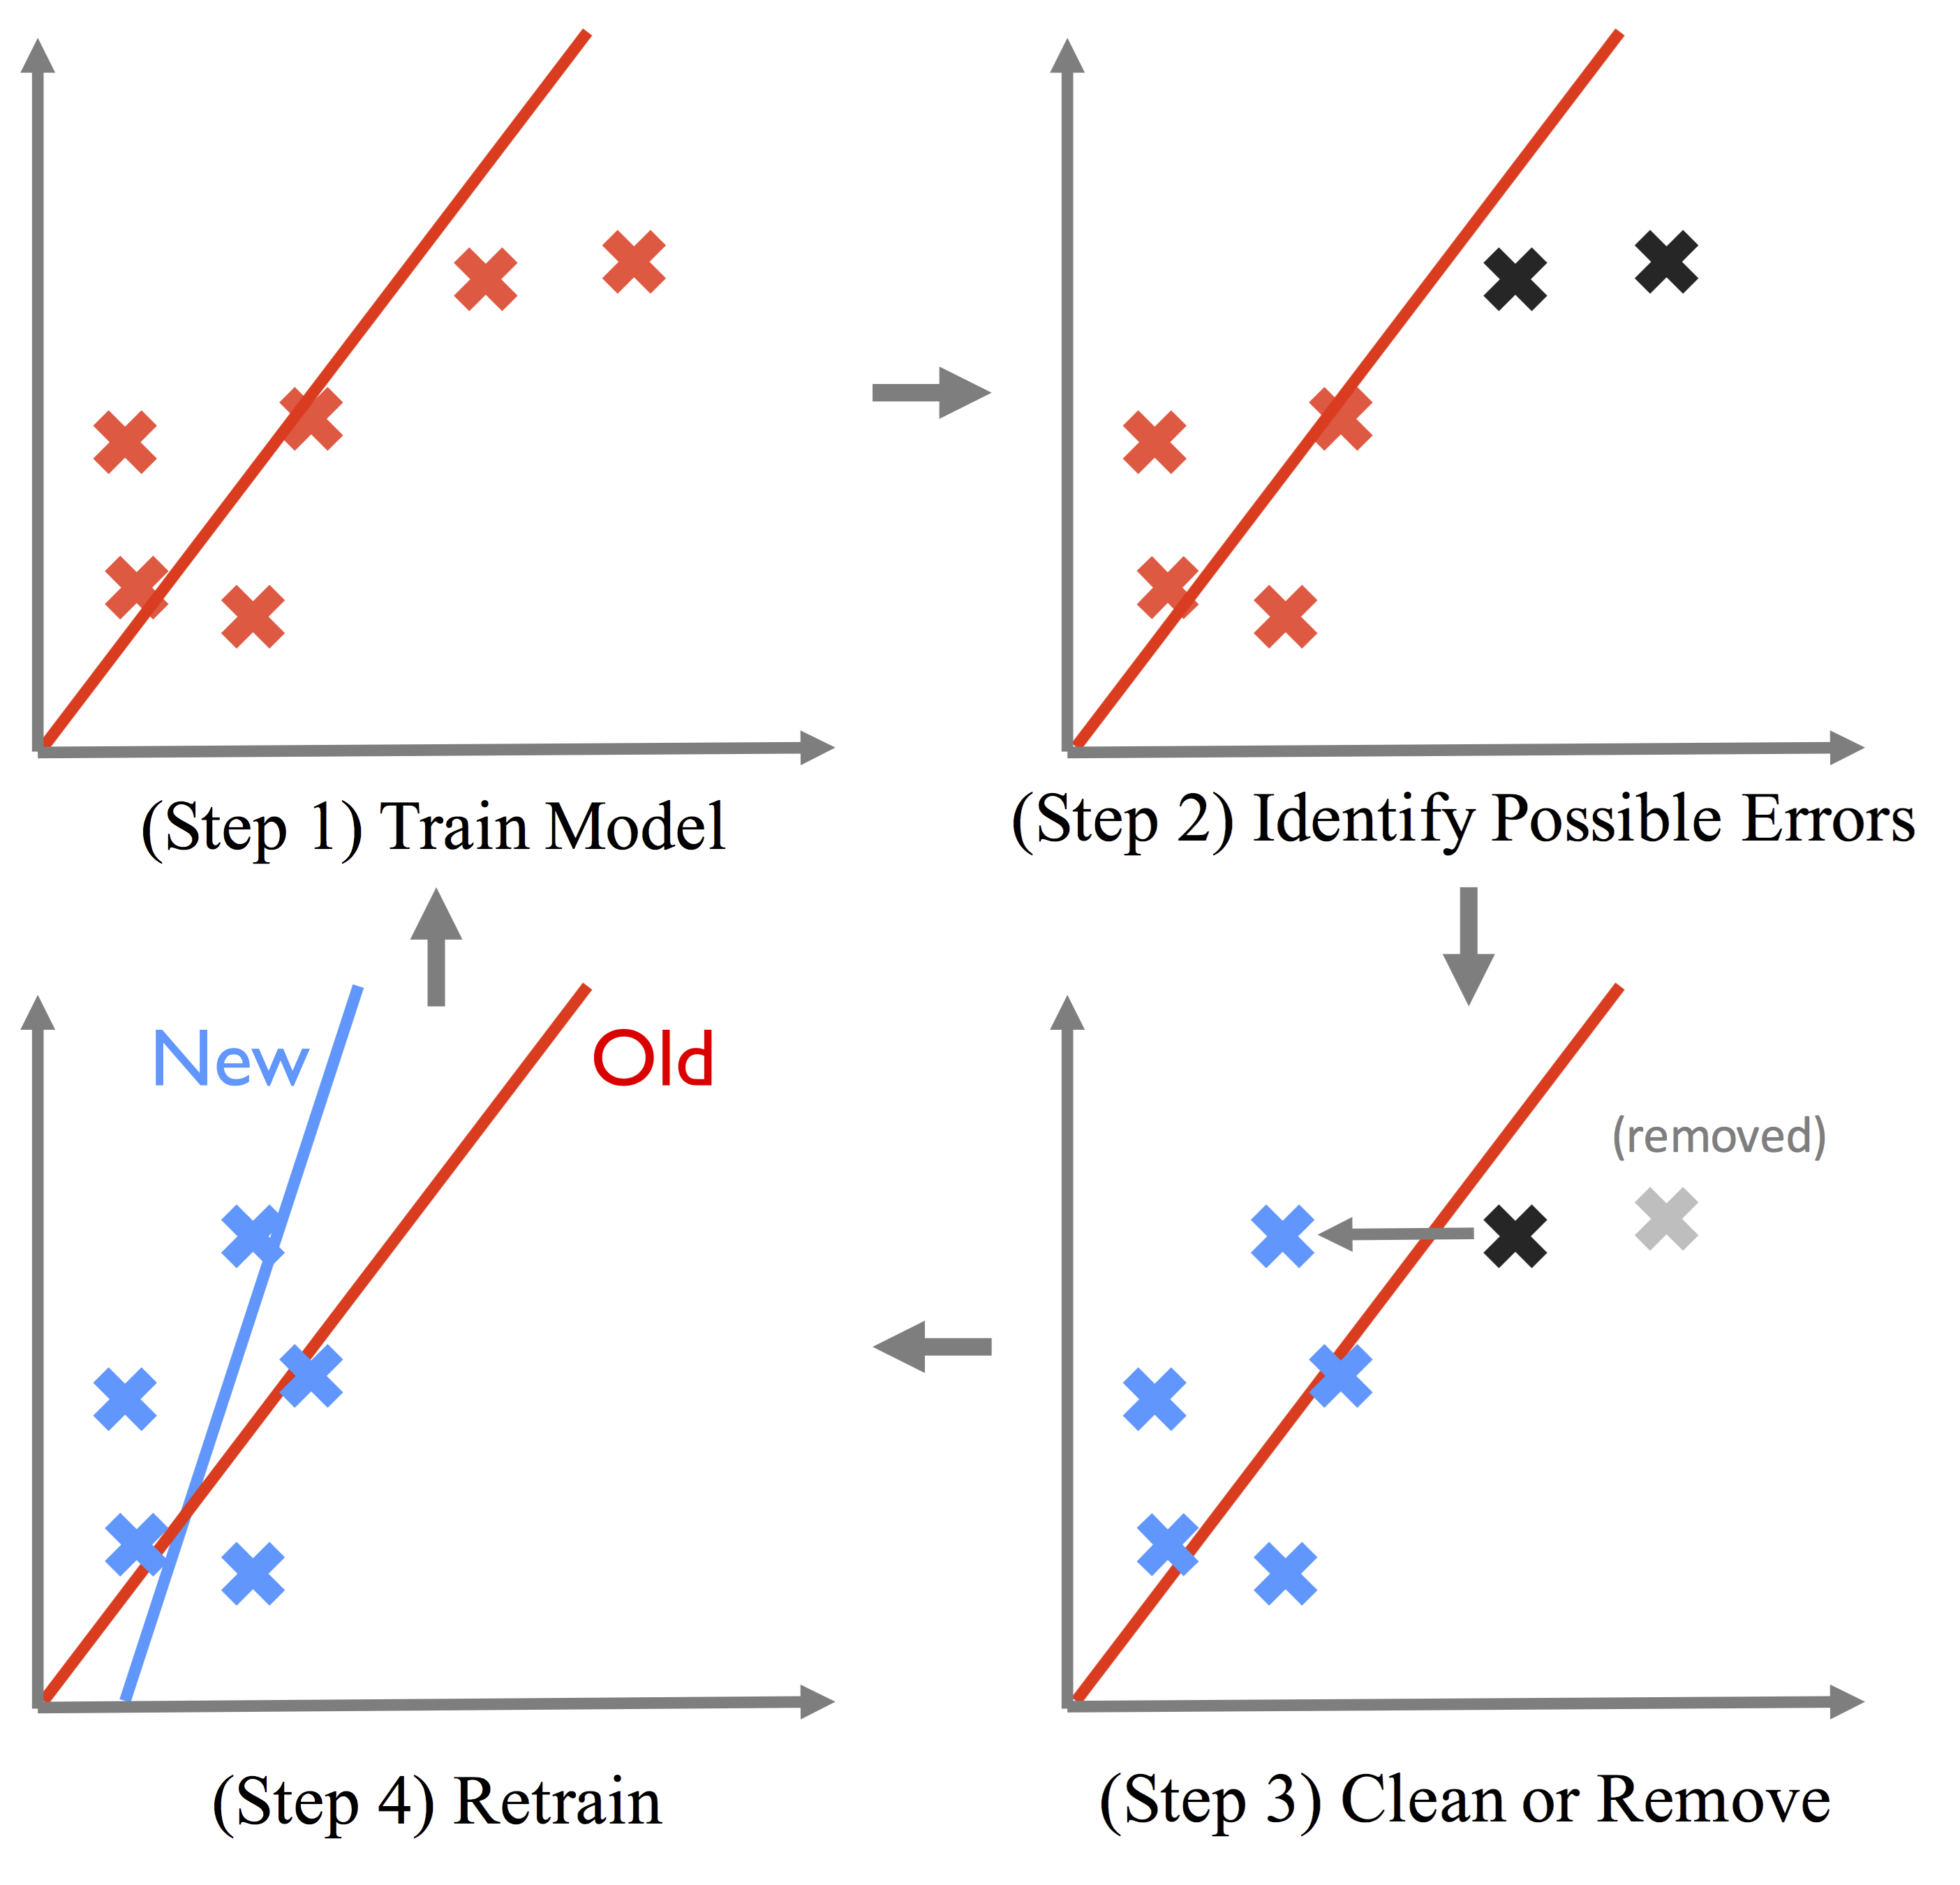
\includegraphics[width=0.8\columnwidth]{figs/update-arch4.png}
 \caption{Model training on dirty data is often an iterative process with four key steps: training, identification, cleaning, and re-training. \label{teaser}}\vspace{-1.5em}
\end{figure}

However, identifying dirty data can be challenging.
In some lucky cases, a record's corruption causes the training to fail (e.g, a NULL value), and thus alerts the analyst to an issue before training.
Unfortunately, there are many types of corruption where the training succeeds yet induces significant inaccuracy in the model.
For example, battery-powered sensors can transmit unreliable measurements when battery levels are low \cite{DBLP:conf/pervasive/JefferyAFHW06}. 
Similarly, data entered by humans can be susceptible to a variety of inconsistencies (e.g., typos), and unintentional cognitive biases~\cite{DBLP:conf/recsys/KrishnanPFG14}.
Detecting such errors often requires training the model and evaluating its prediction accuracy on different subsets of data. 
When a subset of poorly modeled data is identified, the analyst must diagnose whether this is due to model error (i.e., the inherrent error in a statistical model) or data error (i.e., the acutal data are incorrect).
Thus, the process is iterative in a time-consuming train, clean some data, and re-train loop until the analyst is convinced in the model's accuracy (Figure \ref{teaser}).

This iterative process is the de facto standard, but without appropriate care, can lead to several serious statistical issues.
Due to the well-known Simpson's paradox, models trained on a mix of dirty and clean data can have very misleading results even in simple scenarios (Figure \ref{update-arch1}).
Furthermore, if the candidate dirty records are not identified with a known sampling distribution, the statistical independence assumptions required by most training methods are violated. 
The violations of these assumptions can introduce confounding biases.
To this end, we designed \sys which trains predictive models while allowing for iterative data cleaning and has accuracy guarantees.
\sys automates the dirty data identification process and the model update process, thereby abstracting these two error-prone steps away from the analyst.

\sys is inspired by the recent success of progressive data cleaning where a user can gradually clean more data until the desired accuracy is reached~\cite{altowim2014progressive, whang2014incremental, papenbrock2015progressive, gruenheid2014incremental, mayfield2010eracer, DBLP:journals/pvldb/YakoutENOI11, yakout2013don}.
We focus on a popular class of models called convex loss models (e.g., includes linear regression and SVMs) and show that the Simpson's paradox problem can be avoided using iterative maintenance of a model rather than re-training.
This process leverages the convex structure of the model rather than treating it like a black-box, and we apply convergence arguments from convex optimization theory.
We propose several novel optimizations that leverage information from the model to guide data cleaning towards the records most likely to be dirty and most likely to affect the results.

%Consequently, while there is extensive work on progressive data cleaning before analysis, due to the aforementioned problems, existing tools are not suited for application inside the cleaning and training loop.  



%High-dimensional predictive models are highly sensitive to dirty data.
%They rely on learning relationships between features and labels, and systematic data corruption \cite{taylor1982introduction} can mask or even introduce spurious new relationships.
%Furthermore, the high dimensionality of these models can amplify small problems \cite{xiaofeature} resulting in error-prone predictions even when trained on mostly clean data.





%When data cleaning is expensive, it is desirable to apply it \textbf{progressively}, where analysts can inspect early results with only  cleaned.
%Progressive data cleaning is a well studied problem especially in the contex of entity resolution \cite{whang2014incremental, papenbrock2015progressive, gruenheid2014incremental}.
%Increasingly, Active Learning \cite{settles2010active} or other statistical methods are applied to select records or contraint violations to clean in a way that maximizes the information gained \cite{DBLP:journals/pvldb/YakoutENOI11, gokhale2014corleone, yakout2013don}.

%Knowledge of the subsequent data analytics can also .
%While this has been explored in the context of conjuctive queries \cite{DBLP:conf/sigmod/BergmanMNT15} and SQL aggregates \cite{wang1999sample}, it is important to recognize the growing popularity of predictive models in data analytics \cite{bdas, alexandrov2014stratosphere, crotty2014tupleware, hellerstein2012madlib}.
%Predictive models rely on learning relationships between features and labels, and systematic data corruption \cite{taylor1982introduction} can mask or even introduce spurious new relationships.
%Furthermore, the high dimensionality of these models can amplify small problems \cite{xiaofeature} resulting in error-prone predictions even when trained on mostly clean data.

%Straight-forward applications of progressive data cleaning before model training can lead to .

%Suppose $k$ records are cleaned, but all of the remaining dirty records are retained in the dataset.

\noindent To summarize the contributions:
\begin{itemize}[noitemsep]
\item \textbf{Correctness} (Section \ref{model-update}). We show how to update a dirty model given newly cleaned data. This update converges monotonically in expectation. For a batch size $b$ and iterations $T$, it converges with rate $O(\frac{1}{\sqrt{bT}})$. 
\item \textbf{Efficiency} (Section \ref{dist-samp}). We derive a theoretical optimal sampling distribution that minimizes the update error and an approximation to estimate the theoretical optimum.
\item \textbf{Detection and Estimation} (Section \ref{opti}). We show how \sys can be integrated with data detection to guide data cleaning towards records expected to be dirty.
\item The experiments evaluate these components on four datasets with real and synthetic corruption (Section \ref{eval}). Results suggests that for a fixed cleaning budget, \sys returns more accurate models than uniform sampling and Active Learning when systematic corruption is sparse.

%For a 5\%  systematic corruption, \sys cleans 55\% fewer records to achieve the same accuracy as an Active Learning algorithm.
\end{itemize}






